\documentclass{article}
\usepackage{mathtools}
\usepackage[margin=0.95in]{geometry}
%\renewcommand{\familydefault}{\sfdefault}
\usepackage{amssymb}
\usepackage{cancel}
\usepackage{tikz-cd}
\usepackage{tikz}
\usepackage{caption}
\usepackage{pgfplots}
\usepackage{pgf}
\usepackage{centernot}
\usetikzlibrary{arrows,automata}
\usepackage{booktabs}
\usepackage{enumerate}
\usepackage{multirow}
%\usepackage{bbold}
\usepackage{changepage}
\pgfplotsset{compat = newest}
\usepackage{gensymb}
\usepackage[utf8]{inputenc}
\usepackage[english]{babel}
\usepackage{stmaryrd}
\usepackage{xcolor}
\usepackage{listings}
\definecolor{background}{RGB}{255,248,197}
\usepackage{color}
\usepackage{hyperref}
\hypersetup{colorlinks=true, linkcolor=black,
urlcolor=blue, linktoc=all}
\setcounter{MaxMatrixCols}{20}
\usepackage{witharrows}
\usepackage{graphicx}
\usepackage{bm}
\usepackage{tabu}
\usepackage[many]{tcolorbox} %[enhanced,boxrule=0pt, frame hidden, sharp corners, borderline west={3pt}{-1.5pt}{black},breakable]
\usepackage{amsthm}
\usepackage{xfrac}
\usepackage{commath}
\usepackage{dirtytalk}
\usepackage{ytableau}
\newcommand{\inv}{^{-1}}
\newcommand{\qtq}[1]{\quad\text{#1}\quad}
\newcommand{\txt}[1]{\ \text{#1}\ }
\renewcommand{\ker}{\text{ker}}
\newcommand{\coker}{\text{coker}}
\newcommand{\Cor}{\text{Cor}_G(H)}
\newcommand{\ind}{\xrightarrow{d}}
\newcommand{\inp}{\xrightarrow{P}}
\newcommand{\almo}{\xrightarrow{\text{a.s}}}
\newcommand{\vecv}{\vec{v}}
\newcommand{\vecu}{\vec{u}}
\newcommand{\vecw}{\vec{w}}
\newcommand{\zmod}[1]{\Z/ #1 \Z}
\newcommand{\floor}[1]{\lfloor #1 \rfloor}
\newcommand{\lip}{\langle}
\newcommand{\rip}{\rangle}
\DeclareSymbolFont{symbolsC}{U}{txsyc}{m}{n}
\DeclareMathSymbol{\indep}{\mathrel}{symbolsC}{121}
\newcommand{\newpar}{\vspace{8pt}}
\renewcommand{\phi}{\varphi}
\newcommand{\ptwo}{p_\Lambda^{(2)}}
\newcommand{\pthree}{p_\Lambda^{(3)}}
\renewcommand{\epsilon}{\varepsilon}
\renewcommand{\theta}{\vartheta}
\DeclareMathOperator*{\argmax}{arg\,max}
\DeclareMathOperator{\deg}{deg}
\DeclareMathOperator*{\argmin}{arg\,min}
\DeclareMathOperator*{\limeaunf}{limea\"unf}
\newcommand{\Ree}{\text{Re}}
\newcommand{\Imm}{\text{Im}}
\newcommand{\iid}{\stackrel{\text{i.i.d}}{\sim}}
\newcommand{\rank}{\text{rank}}
\newcommand{\Span}{\text{span}}
\newcommand{\Int}{\text{Int}}
\newcommand{\Clos}{\text{Clos}}
\newcommand{\ideal}{\mathfrak{A}}
\newcommand{\idm}{\mathfrak{m}}
\newcommand{\idn}{\mathfrak{n}}
\newcommand{\idp}{\mathfrak{p}}
\newcommand{\idq}{\mathfrak{q}}
\newcommand{\limty}{\lim_{n\to\infty}}
\newcommand{\seq}[1]{(#1_n)_{n\geq1}}
\newcommand{\leteps}{\text{Let } \varepsilon > 0}
\renewcommand{\char}{\text{char}}
\newcommand{\mb}[1]{\bm{#1}}
\newcommand{\nil}{\text{nil}}
\newcommand{\code}[1]{\texttt{#1}}
\newcommand\bigzero{\makebox(0,0){\text{\huge0}}}
\renewcommand{\div}{\text{div}}
\newcommand{\R}{\mathbb{R}}
\newcommand{\N}{\mathbb{N}}
\newcommand{\C}{\mathbb{C}}
\renewcommand{\P}{\mathbb{P}}
\newcommand{\F}{\mathcal{F}}
\newcommand{\Z}{\mathbb{Z}}
\newcommand{\Q}{\mathbb{Q}}
\newcommand{\I}{\mathbb{I}}
\newcommand{\T}{\mathbb{T}}
\newcommand{\E}{\mathbb{E}}
\renewcommand{\S}{\mathbb{S}}
\newcommand{\zd}{\text{zd}}
\newcommand{\normal}{\vartriangleleft}
\newcommand{\Aut}{\text{Aut}}
\newcommand{\Inn}{\text{Inn}}
\newcommand{\ds}{\displaystyle}
\newcommand{\Vol}{\text{Vol}}
\newcommand{\sip}{(\ \ \mid\ \ )}
\newcommand{\intfin}{\int_{-\infty}^{\infty}}
\newcommand{\sumi}[1]{\sum_{i=1}^{#1}}
\newcommand{\ren}[1]{\mathbb{R}^{#1}}
\newcommand{\con}[1]{\mathbb{C}^{#1}}
\newcommand{\chisq}[1]{\chi^2_{#1}}
\newcommand{\orthcomp}{^{\perp}}
\newcommand{\im}{\text{im}}
\newenvironment{graytext}{\color{gray}}{\ignorespacesafterend}
\newcommand{\cov}{\text{cov}}
\newcommand{\var}{\text{var}}
\renewcommand{\l}{\left}
\renewcommand{\r}{\right}
\definecolor{codegreen}{rgb}{0,0.6,0}
\definecolor{codegray}{rgb}{0.5,0.5,0.5}
\definecolor{codepurple}{rgb}{0.58,0,0.82}
\definecolor{backcolour}{rgb}{0.95,0.95,0.92}
\mathtoolsset{showonlyrefs} 
\usepackage[utf8]{inputenc}
\setlength\parindent{0pt}

\lstdefinestyle{mystyle}{
    backgroundcolor=\color{backcolour},   
    commentstyle=\color{codegreen},
    keywordstyle=\color{magenta},
    numberstyle=\tiny\color{codegray},
    stringstyle=\color{codepurple},
    basicstyle=\ttfamily\footnotesize,
    breakatwhitespace=false,         
    breaklines=true,                 
    captionpos=b,                    
    keepspaces=true,                 
    numbers=left,                    
    numbersep=5pt,                  
    showspaces=false,                
    showstringspaces=false,
    showtabs=false,                  
    tabsize=2
}

\lstdefinestyle{python2}{
    language=Python,
    basicstyle=\ttfamily\small,
    keywordstyle=\color{blue},
    commentstyle=\color{gray},
    stringstyle=\color{red!60!black},
    showstringspaces=false,
    frame=single,
    numbers=left,
    numberstyle=\tiny\color{gray},
    tabsize=4,
    breaklines=true,
}

\title{\textbf{\textsf{Stat 175: Homework 1}}}
\author{\textsf{Prof. Morgane Austern}}
\date{\textsf{Spring 2026}}

\begin{document}

\maketitle

Please submit your solutions to Gradescope by \textbf{Wednesday, February $4^{\text{th}}$, 11:59pm}.

\begin{tcolorbox}[colback = gray!16, enhanced, boxrule=0pt, frame hidden, sharp corners, borderline west={3pt}{-1.5pt}{black!80},breakable]
\textbf{Exercise 1 (Markov Chains).} The following network represents the road network between seven different cities. There is an edge between two cities if there is a road between them. For example, there is a road between cities 1 and 2, but not between cities 1 and 5. We call $i$ and $j$ neighbors if there is an edge between them. We write by $\text{deg}(j)$ the number of neighbors that the city $j$ has. For example, $\text{deg}(1) = 3$. A traveler is driving from town to town. At time 0,
they start at the random city $X_0 \sim \pi$, where we denote by $X_j$ the city in which the driver wakes up on the $j^{\text{th}}$ day. Each day the driver then drives to a new city chosen at random among all the cities that are connected to $X_j$. This new city is written as $X_{j+1}$. For example, if $X_j = 1$ then they will drive either to city 2, 3, or 6, and thus $X_{j+1} \sim \text{Unif}\{2, 3, 6\}$. We call $(X_j)$ a \textit{random walk} on the network.

    \begin{center}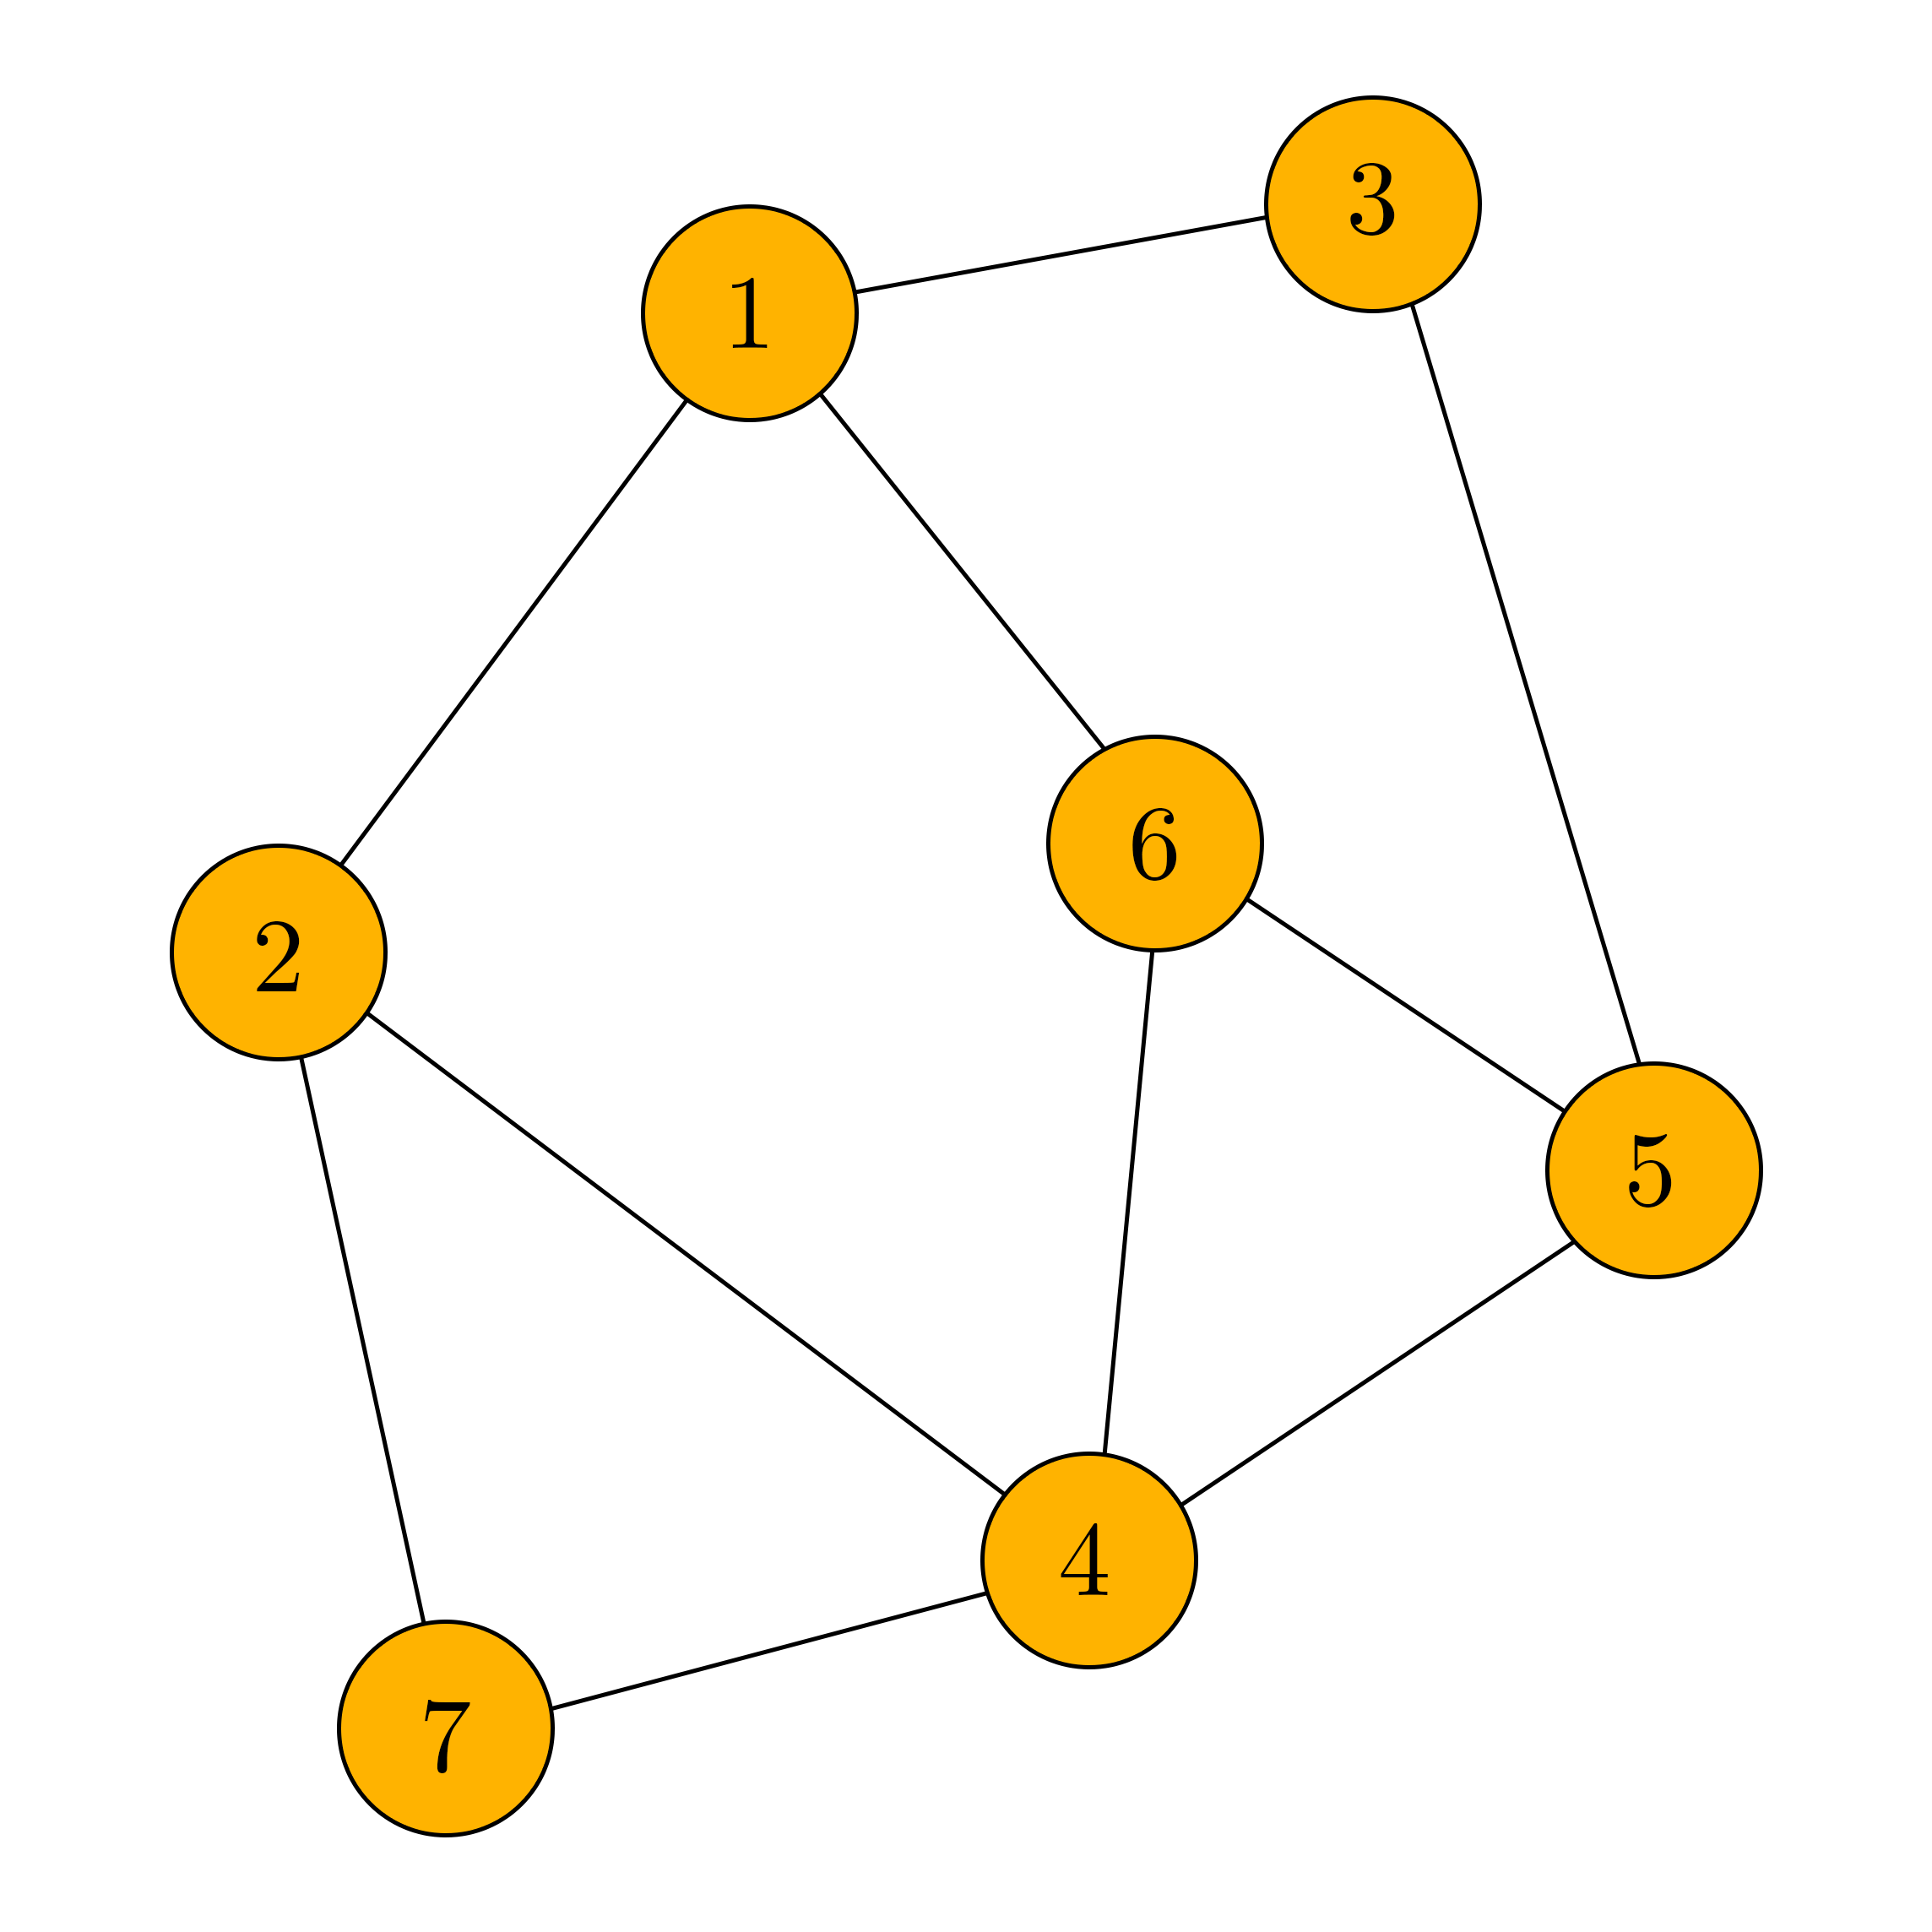
\includegraphics[width=0.4\linewidth]{Figures/hw1_graph1.png}\end{center}
\begin{enumerate}[$(a)$]
    \item Prove that $(X_j)$ is a Markov chain.
    \item What is the transition probability matrix of this Markov chain? Denote this
    transition matrix by $P$.
    \item Prove that the stationary distribution is given by $\pi(j) = \frac{\text{deg}(j)}{20}$.
    \item We say that the Markov Chain is reversible if $\pi(i)P_{ij} = \pi(j)P_{ji}$ for all $i, j$. Prove that the Markov Chain is reversible. 
    \item Suppose we modify the walk like so: at each step, with probability $\alpha \in (0,1)$, the driver stays in the current city, and with probability $1-\alpha$, they move to a uniform neighbor as before. Does this change the stationary distribution? Provide a formal proof.
    
(\textit{It might have been a while since you've read about Markov chains. For
a reminder,} \href{https://www.statslab.cam.ac.uk/~rrw1/markov/M.pdf}{click here}).
\end{enumerate}
\end{tcolorbox}

\pagebreak

\begin{tcolorbox}[colback = gray!16, enhanced, boxrule=0pt, frame hidden, sharp corners, borderline west={3pt}{-1.5pt}{black!80},breakable]
\textbf{Exercise 2 (Linear Algebra).} A matrix $(A_{ij})$ is called an \textit{adjacency matrix} of a network if 
\begin{enumerate}[$(i)$]
    \item for all $i$, $A_{i, i} = 0$.
    \item for all $i \neq j$, $A_{i, j} = \begin{cases}
        1, & \text{ there exists an edge between vertices $i$ and $j$}\\
        0, & \text{ otherwise.}
    \end{cases}$
\end{enumerate}
Let $D = \text{diag}\l(\text{deg}(i)\r)$ be the diagonal matrix such that $D_{i, i}$ is the degree of vertex $i$. The matrix $L := D - A$ is called the \textit{Laplacian matrix} of the graph. Consider the following graph:
    \begin{center}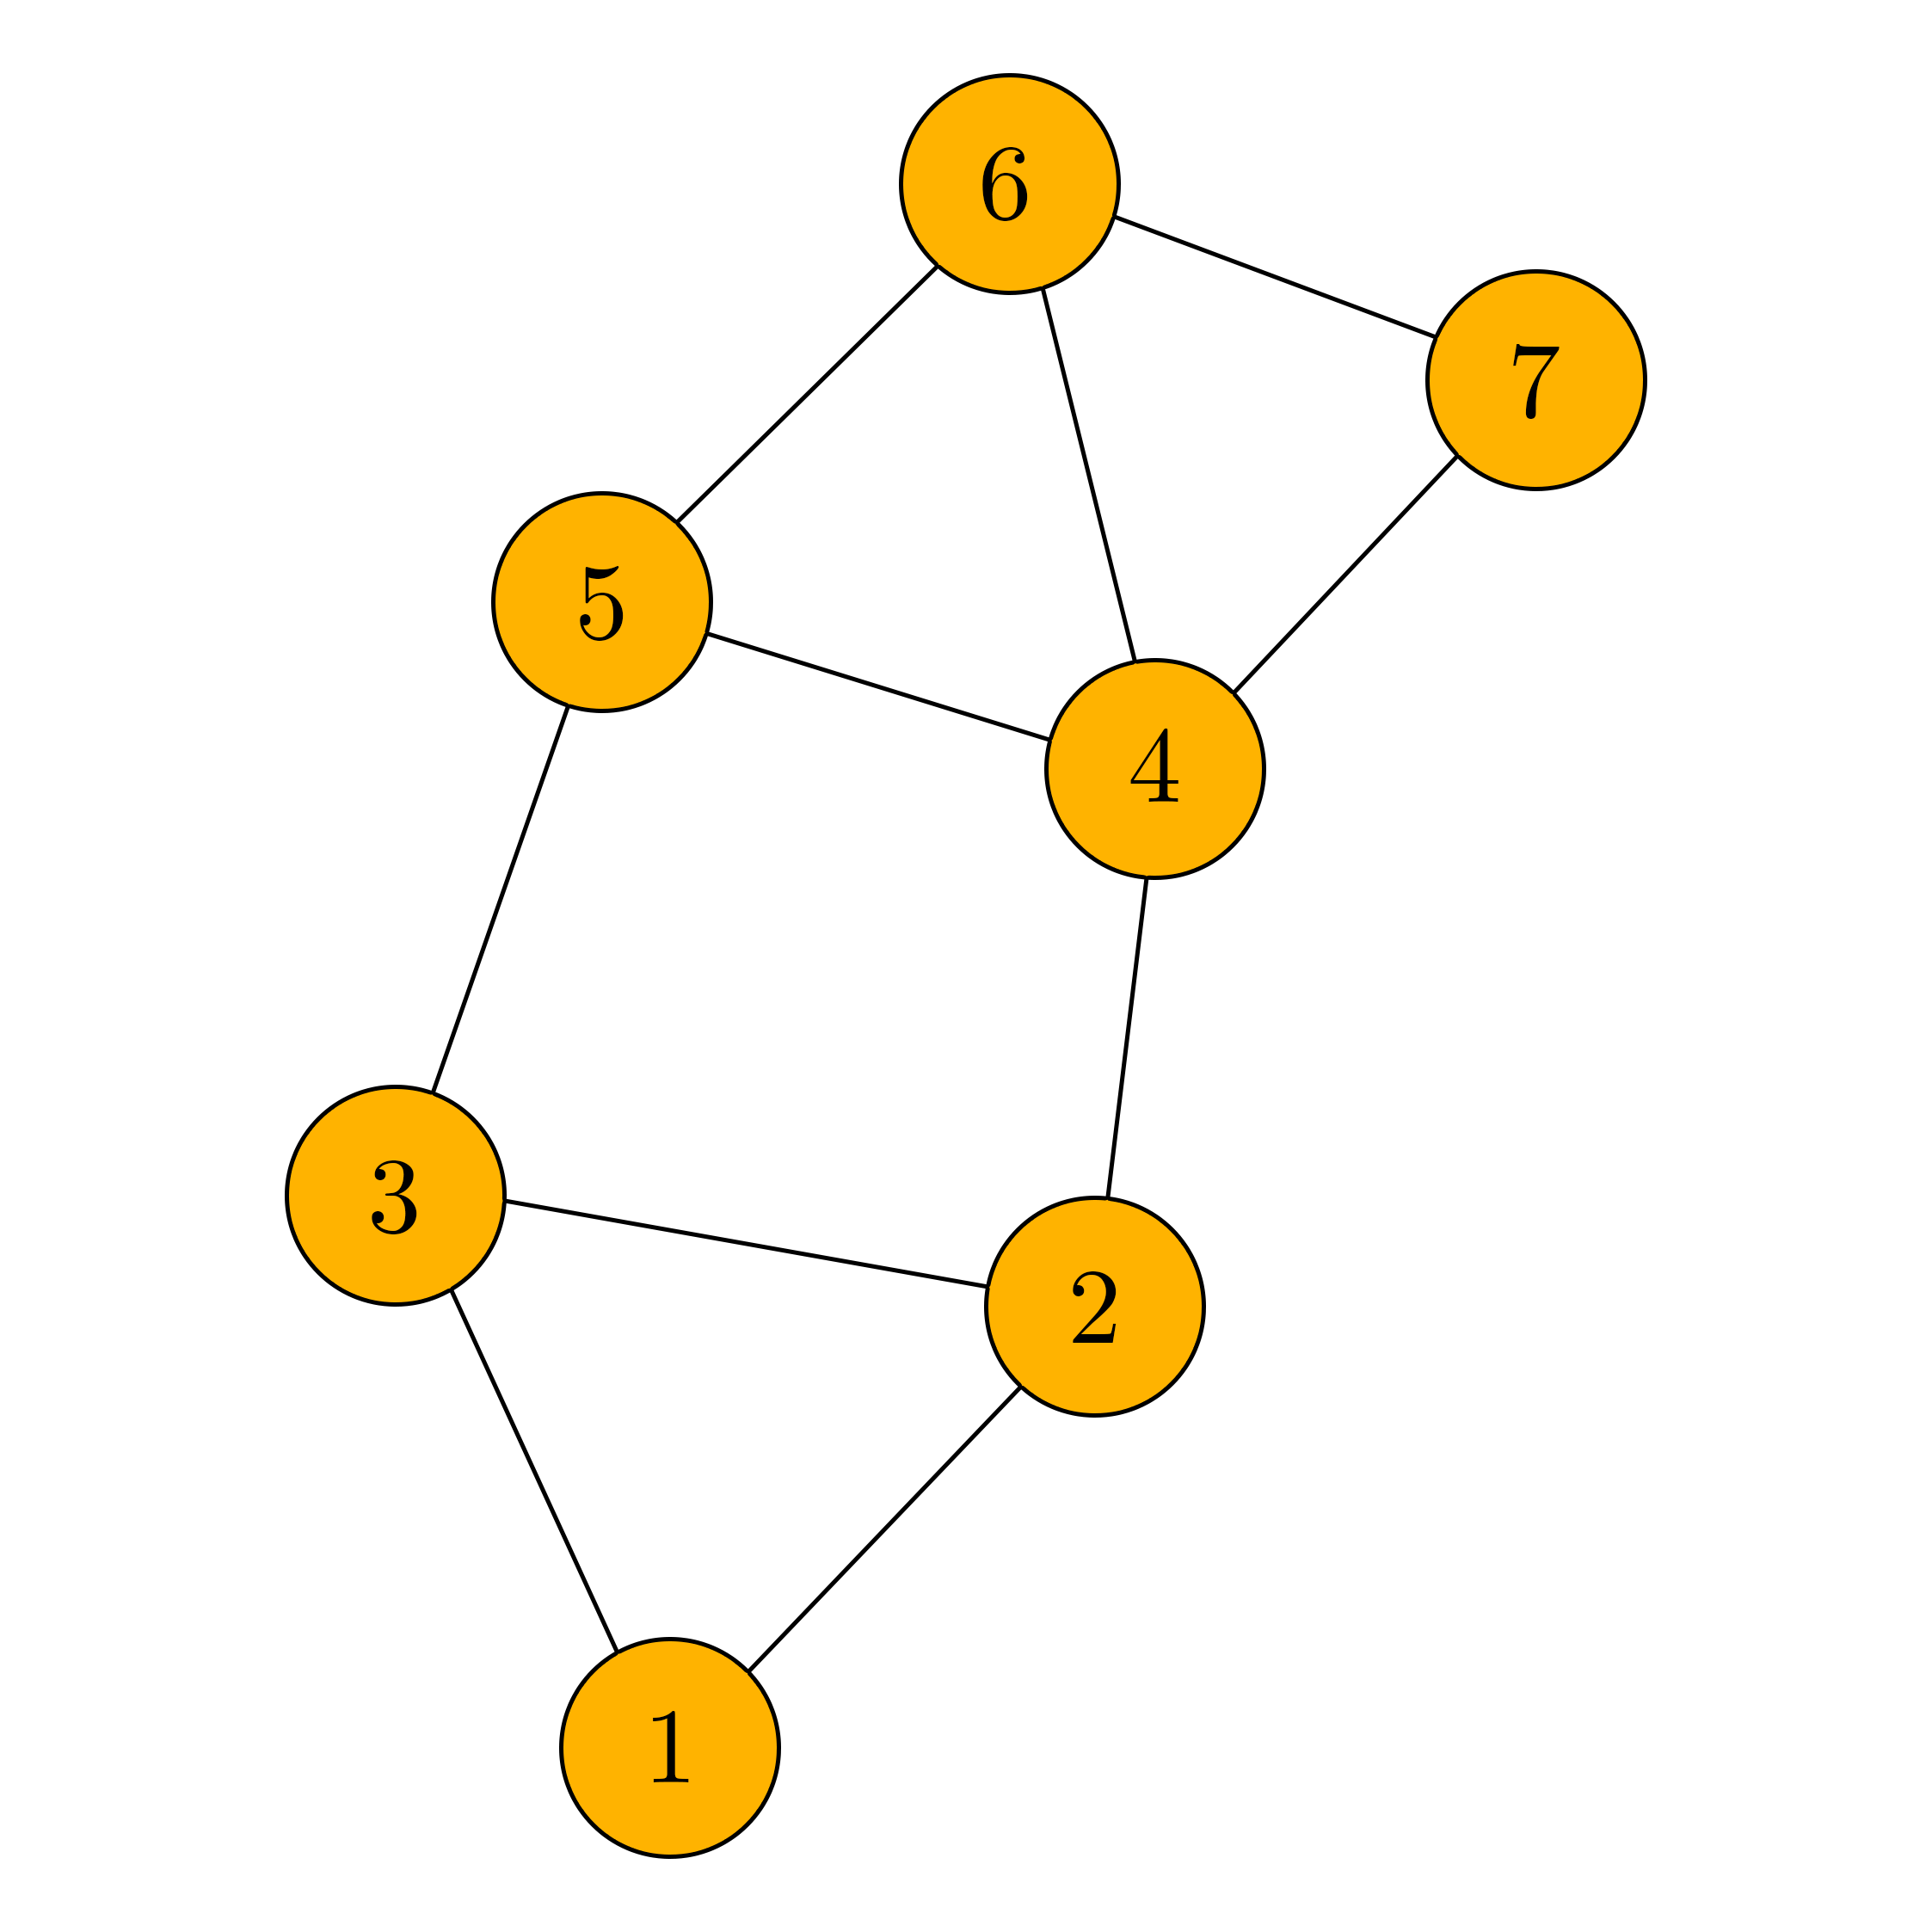
\includegraphics[width=0.4\linewidth]{Figures/hw1_graph2.png}\end{center}

\begin{enumerate}[$(a)$]
    \item What is the adjacency matrix of the network? What is the Laplacian matrix of the network?
    \item Compute the eigenvalues of $L$ (feel free to use Python). Remark that the vector $\bm1 = (1, \hdots, 1)$ is an eigenvector.
    \item Consider a general undirected graph. Prove that for any vector $x\in\R^n$, the quadratic form satisfies
    \begin{align*}
        x^\intercal Lx = \sum_{(i, j) \in E}(x_i - x_j)^2.
    \end{align*}
    \item Use this identity to prove that $L$ is positive semi-definite and that the smallest eigenvalue is always $\lambda_1 = 0$.
    \item Let $\lambda_2$ be the second smallest eigenvalue of $L$. Prove that if the graph $G$ is disconnected, then $\lambda_2=0$. (\textit{Hint: Consider the vector $x$ that is constant on one connected component and zero elsewhere}).
\end{enumerate}
\end{tcolorbox}


\begin{tcolorbox}[colback = gray!16, enhanced, boxrule=0pt, frame hidden, sharp corners, borderline west={3pt}{-1.5pt}{black!80},breakable]
\textbf{Exercise 3 (Statistical Inference).} Let $(X_i)$ be a sequence of i.i.d. random variables with the probability density function given by 
\begin{align*}
    f(x) := \frac{1}{2\sigma}e^{-|x|/\sigma}.
\end{align*}
\begin{enumerate}[$(a)$]
    \item Write out the log-likelihood function $\ell(X_1, \hdots, X_n)$. 
    \item What is the maximum likelihood estimator (MLE) of $\sigma$? Denote it by $\hat\sigma$.
    \item Is the MLE consistent? Prove your answer.
\end{enumerate}
\end{tcolorbox}


\begin{tcolorbox}[colback = gray!16, enhanced, boxrule=0pt, frame hidden, sharp corners, borderline west={3pt}{-1.5pt}{black!80},breakable]
\textbf{Exercise 4 (Probability Theory).} Let $(U_i) \iid \text{Unif}(0, 1)$ be a sequence of i.i.d. random variables and $W : [0, 1]^2 \to [0,1]$ a continuous (and measurable, if you recall what that means) function. Let $(a_{i,j})$ be a sequence of Bernoulli random variables drawn in the following way:
\begin{align*}
    a_{i, j} \sim \text{Bern}\l(W(U_i, U_j)\r).
\end{align*}
Define $d_i := \sum_{j\neq i \leq n}a_{ij}$. 
\begin{enumerate}[$(a)$]
    \item Compute $\E\l[d_i \mid U_i\r]$ and $\E\l[d_i\r]$ for each vertex $i$.
    \item Compute $\var\l(d_i \mid U_i\r)$ and $\var(d_i)$ for each vertex $i$.
    \item Compute $\text{cov}(d_i, d_j)$ for each vertex pair $i, j$.
    \item What is the limit of $\dfrac{d_1}{n}$ and $\dfrac{d_2}{n}$? Do they converge to the same quantity? Does $d_1$ satisfy some form of CLT? Justify this.
    \item What is the limit of $\dfrac{\sum_{i\leq n}d_i}{n^2}$?
\end{enumerate}
\end{tcolorbox}







\end{document}